\chapter{Discrete Fourier transform and fast Fourier transform}
\section{Discrete Fourier transform}
	The \de{Discrete Fourier Transform} (DFT) is different from the previously discussed Discrete Time Fourier Transform (DTFT); in this second case in fact the variable $\omega$, expressed in radians, is real evaluated, while in the discrete Fourier transform. Working instead with the \dft we compute a transform for a finite number of frequency samples $\omega_k \ [rad]$ with $k=0,\dots, N-1$: with this definition we can consider the DFT as a sampling of the transform in the frequency domain. In this case the discrete transform can be computed as
	\begin{equation} \label{eq:ft:dft}
		X(k) = \sum_{n=0}^{N-1} x(n) e^{-j \frac{2\pi}{N}kn} \sum_{n=0}^{N-1} x(n) W_N^{kn} \qquad \forall \ k = 0,1,\dots, N-1
	\end{equation}
	where the term $W_n^{kn}$ is referred as the \textbf{twiddle factor}.
	
	In a practical way the \dft is a sampling of the zeta transform of $N$ samples $\omega_k$ equispaced on the complex unit circle of the $\mathscr Z$ transform of the signal. Increasing the number of $N$ we decrease the \textit{distance} of $\omega_k$ and for $N\rightarrow\infty$ the DFT converges to the discrete-time Fourier transform.
	
	The \dft is not an approximated version of the DTFT, in fact for the same frequency $\omega_k$ the values are the same, but it's only a pure sampling of the continuous transform. \vspace{3mm}
	
	The \dft, in this sense, allow to estimate automatically (that can in fact be computed by machines) the transform of generic non deterministic signals. In practise we don't use the \dft but the \de{Fast Fourier Transform}, a class of complementary algorithms that allows to compute the transform in a faster way (respect to the DFT definition). \vspace{3mm}
	
	Considering the equation \ref{eq:ft:dft} we can see that this expression maxes sense only for signal with a finite number of sample (points); in particular to correctly compute the \dft the number of samples for the sequence $x(n)$ is truncated to $N$ (and having less samples than the decided resolution for $N$, we have to decrease the number of sampling in the transform). The number of frequency samples has to be equal or greater to the number of signal samples.
	
	\paragraph{Inverse Discrete Fourier Transform} In order to compute instead the \de{Inverse Discrete Fourier Transform} (IDFT) we can use the following definition:
	\begin{equation} \label{eq:ft:idft}
		x(n) = \frac 1 N \sum_{k=0}^{N-1} X(k) e^{j\frac{2\pi}{N} kn} \qquad \forall \ n = 0,1,\dots,N-1
	\end{equation}
	This is indeed the inversion of the linear problem of the equation \ref{eq:ft:dft} considering that there are $N$ equations ($X(i)$ for $i=0,\dots, N-1$) having $N$ samples each. Considering that the coefficients are $W_N^{kn}$ we can define the vectorial form of equation \ref{eq:ft:dft} as $\boldsymbol X = W \boldsymbol x$ and so $\boldsymbol x = W^{-1} \boldsymbol X$ (where $K \in \mathds R^{N\times N}$ is the coefficient matrix that's for sure non singular).
	
\subsection{Time aliasing problem}
	Given an arbitrary sequence $x(n)$ whose discrete time Fourier transform is expressed as $X(e^{j\omega})$. By computing the inverse discrete time Fourier transform we can simply reconstruct the original signal, however if we consider the \dft  $X(k)$ of the signal and we invert the result we see that the reconstructed signal $\tilde x(n)$ that's equal to the original signal only for a finite number of samples, and in particular $\tilde x(n) = x(n)$ only for $n=0,1,\dots, N-1$ and only if $N$ is longer then the input sequence length.
	
	Applying the definition of inverse \dft (eq. \ref{eq:ft:idft}) we can see that the reconstructed signal $\tilde x(n)$ must be necessarily a periodic function in time (due  to the linear combination of the twiddle factors) and so
	\[ \tilde x(n) = \frac 1 N \sum_{k=0}^{N-1} X(k) e^{j\frac{2\pi}{N} kn} = \sum_{r=-\infty}^\infty x(n-rN) \]
	
	Given $L$ the number of non-zero samples of the original signal $x(n)$ and compute a \dft with $N$ samples; if $N<L$ then we have the time aliasing problem, while we don't see this problem for $N\geq L$. The number of overlapping samples is equal to $L-N$. If we want only to perform a spectrum analyses (that wont' be followed by a reconstruction) this relations are not necessary (and we can choose any value of $N$).
	
	\begin{SCfigure}[2][bht]
		\centering 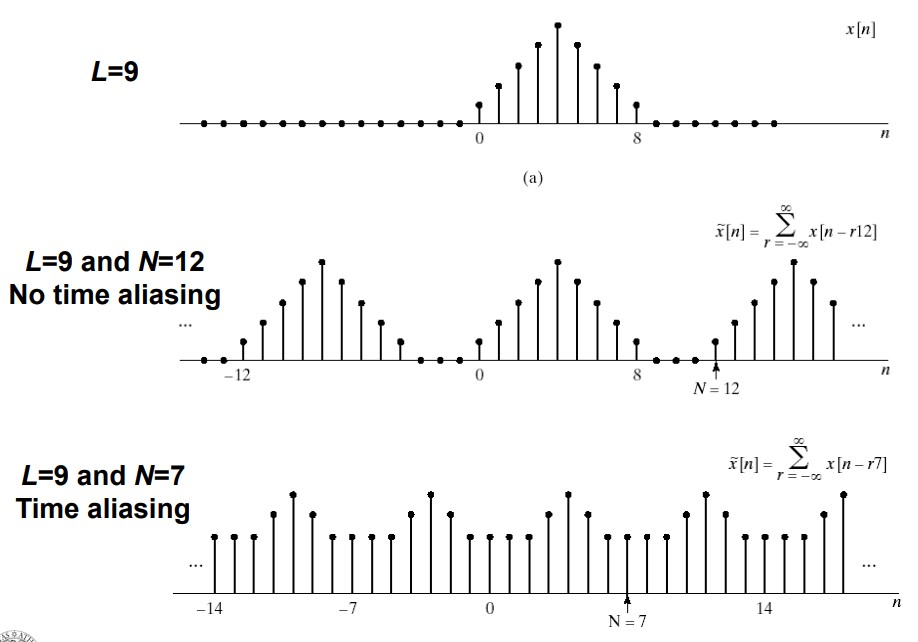
\includegraphics[width=8.5cm]{time-aliasing}
		\caption{original sequence $x(n)$ (on top) with $L=9$ and reconstructed signals $\tilde x(n)$ changing $N$ to $12 (>L)$ and $7 (<L)$. }
	\end{SCfigure}
	
	This concept is the dual result of the spectral replicas that are present in the sampling process on the time domain (in this case we are sampling in the frequency domain and so we have aliasing replicas in time domain).

\subsection{Properties}
	The \dft is a \textbf{linear operator}, in fact given two sequences $x_1(n),x_2(n)$ having discrete transforms $X_1(k),X_2(k)$ then
	\[ a x_1(n) + b x_2(n) \quad \mapsto \quad a X_1(k) + bX_2(k) \qquad \forall a,b \in \mathds R \]
	In particular if the two sequences have different length (for example $N_1 < N_2$) a number of $|N_2-N_1|$ should be added to the shorter sequence, so by doing a \textbf{zero padding}.
	
	We can also consider the \textbf{circular shifting} property that given a sequence $x(n)$ of $N$ samples with \dft $X(k)$, then given a time shift of $m\in \mathds Z$ samples in time determines a sequence
	\[ \tilde x(n-m) \ n = 0,\dots, N-1\quad \mapsto \quad X(k) e^{-j \frac{2\pi k}{N}m} \]
	where $\tilde x(n)$ is the \textit{infinite repetition} of the signal $x(n)$ (concatenation of the same signal). If the original signal $x(n)$ is real evaluated, then $\Re \{ X(k) \} = \Re \{ X(N-k) \}$ (even symmetry on the real axis) and $\Im \{X(k)\} = - \Im \{X(N-k)\}$. 

	Another property is the \textbf{circular convolution} and so given two signals $x_1,x_2 \mapsto X_1,X_2$, then
	\begin{equation}
		x_3(n):=x_1(n) * x_2(n) \mapsto X_1(k)X_2(k)  = X_3(k) \qquad k = 0,\dots, N-1
	\end{equation}
	By computing now the inverse \dft (with $N$ samples) on this result the result that we get is not the original signal $x_3(n)$, but $\tilde x_3(n)$ that's equal to $\tilde x_1(n) * x_2(n) = x_1(n) * \tilde x_2(n)$ (and this is due to the periodicity of the signals). Considering that this convolution is performed over $N$ samples, this operation is now called \textbf{circular convolution} $x_1(n) \circconv{N} x_2(n)$ defined as
	\begin{equation}
		x_1(n) \circconv{N} x_2(n) : = \sum_{m=0}^{N-1} x_1(m) \tilde x_2(n-m)
	\end{equation}
	Considering that $x_1$ consists of $L$ values, while $x_2$ consist of $P$ point, than if the \dft sampling point is equal to $N \geq L + P - 1$ then $x_1(n) * x_2(n) = x_1(n) \circconv N x_2(n)$, otherwise the result of the linear convolution and the circular one can be different.
	
	\paragraph{Impulse response} As described at page \pageref{sec:impulseresponse}, we denote as $h(n)$ the impulse response of a system and in case of a finite impulse response (FIR) one we have that $h(n) \neq 0$ for $n=0,\dots,P-1$. Assuming to have an input sequence $x(n)$ fed into the system will determine an output sequence $y(n)$ that's equal to
	\[ y(n) = x(n) * h(n) \] 
	
	Considering that also the input $x(n)$ as a finite number $L$ of samples, then the length of the convolution $y(n)$ will be different from zero for $n=0,\dots, L+P-2$ (and so it present $L+P-1$ samples). In general a way to solve this kind of problem can be solved in the frequency domain. Considering the discrete time Fourier (DTFT) transform $\F$, known the transforms $H(e^{j\omega}), X(e^{j\omega})$ of the system impulse response and input sequence, than the output can be computed as
	\[ Y(e^{j\omega}) = H(e^{j\omega}) X(e^{j\omega}) \qquad \xrightarrow{\mathscr{F}^{-1}} \quad y(n) \]
	In general this operation using the \dft (DFT), that's practically what happens, is more complex. Given the two discrete transform $X(k),H(k)$ of both the input and the impulse response, we can compute the output frequency response $Y(k) = H(k) X(k)$ that can be inverted to $y(n)$. In order to do perform this operation correctly (and not losing information due to time aliasing) the two transform have to be computed doing a zero padding for $x(n)$ with $P-1$ zero and a padding of $L-1$ zero for $h(n)$: in this case we are sure that the product $X(n)H(n)$ has a number of samples $N = L+P$ that's greater than the $L+P-1$ due to the convolution.

\section{Fast Fourier transform}
	The \de{\fft}, as already stated, is not the same as the \dft but represent a class of algorithms that are implemented to compute the Fourier transform in a \textit{faster} way (by doing less mathematical computation than the original statement).
	
	Starting from the definition on page \pageref{eq:ft:dft} of the \dft we can see that to determine the spectrum we need to perform $N-1$ complex addition and $N$ complex multiplications for each spectral sample, and so the full number of operation to perform is
	\[ N(N-1) \textrm{ complex addition} \quad + \quad N^2 \textrm{ complex multiplication} \]
	Considering that computers can't handle complex number but only real values, it means that one complex multiplication corresponds to 4 multiplications and 2 additions in the real domain (and one complex addition corresponds to 2 real additions). We can see that in general the order of complexity of the \dft is equal to
	\[ \mathcal O \big(N^2\big)\]
	
	The \fft allow to reduce the order of complexity of the operation op to the value $\mathcal O \big(N \log_2 N\big)$ (that's the ideal target value for all the algorithms) then $N$ is a power of 2, and so can be rewritten as $N = 2^\nu$ with $\nu \in \mathds N$. When this conditions is not met, usually the input sampled signal is subdivided in sequences that met the condition, perform the FFT and then recombine the result.
	
\subsection{Decimation in time FFT}
	The basic idea of the \de{decimation in time} DIT \fft algorithm is to recursively decompose the original DFT into more transforms with smaller number of points obtained through bisection.
	
	Considering for example the sequence $x(n) \neq 0$ for $n=0,\dots, N_1$ with $N = 2^\nu$, we can compute two subsequence determined by the sample in even $x_e$ and odd $x_o$ positions, having $N/2$ samples each:
	\[ \underbrace{x(0),x(2),\dots,x(N-2)}_{x_e(n) = x(2r)} \qquad \underbrace{x(1), x(3),\dots, x(N-1)}_{x_o(n) = x(2r + 1)}  \]
	
	Based on the definition (eq. \ref{eq:ft:dft}) of the \dft, we can compute the transform as
	\[ X(k) = \sum_{n=0}^{N-1} x(n) W_N^{kn} = \sum_{r=0}^{\frac N 2 - 1 } x(2r) W_N^{2rk} + \sum_{r=0}^{\frac N 2 - 1} x(2r+1) W_N^{(2r+1)k} \]
	where $W_N = e^{-j\frac{2\pi}{N}}$ is the twiddle factor. We can see that $W_N^2 = W_{N/2}$, in fact
	\[ W_N^2 = e^{-j\frac{2\pi}{N} 2 } = e^{-j\frac{2\pi}{N/2} } = W_{N/2} \]
	and so the previous expression can be rewritten as
	\[ \begin{aligned}
		X(k) & =  \sum_{r=0}^{\frac N 2 - 1 } x_e(r) W_{N/2}^{rk} + W_{N}^k  \sum_{r=0}^{\frac N 2 - 1 } x_o(r) W_{N/2}^{rk} \\ & = X_e(n) + W_N^k X_o(k)  
	\end{aligned} \qquad \qquad \qquad k = 0,\dots,N-1\]
	We can now see that the first sum corresponds to the \dft of the original signal computed only on the even position of $x(t)$, while the second sum corresponds to the odd elements. We can see that computing the transforms $X_e(k),X_o(k)$ requires a number of operation proportional to $(N/2)^2 = N^2/4$, requiring so $1/4$ of the original operations to perform the \textit{pure} transform $X(k)$. If we neglect the time computation of performing the addiction of $X_e+X_o$, than the overall number of operation is
	\[ X_e(k) + X_o(k) \propto \frac{N^2}{4} + \frac{N^2}{4} + N = \frac{N^2}{2} + N \leq N^2 \]
	where the last inequality is always verified for $N>2$.
	\begin{SCfigure}[2][bht]
		\centering 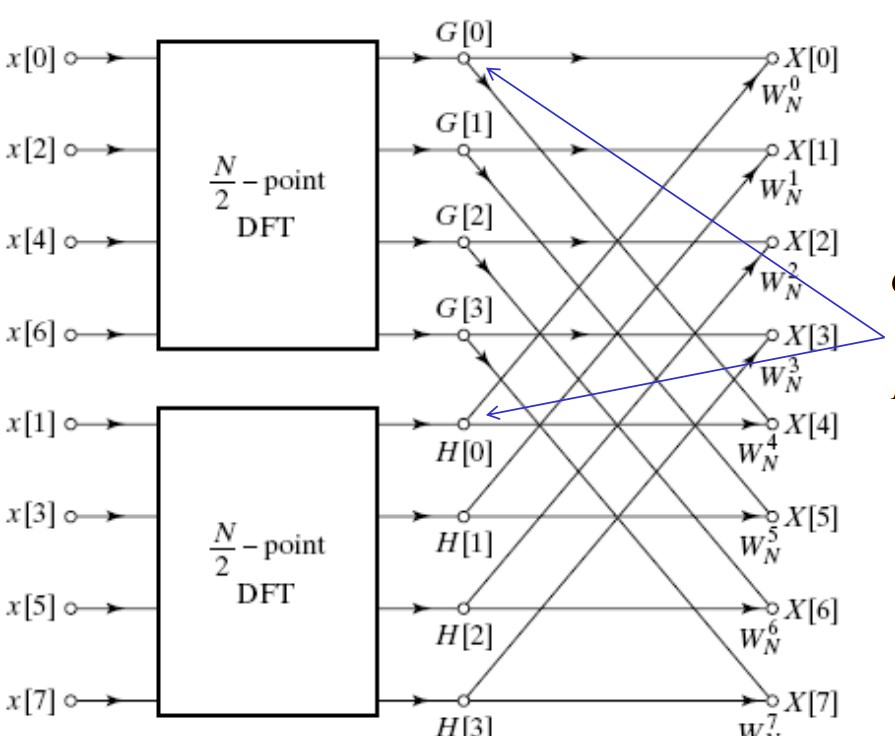
\includegraphics[width=6cm]{fft-dec-graph}
		\caption{graph representing the computation that are needed to be performed to compute the fast Fourier transform using the decimation in time algorithm for $N=8$ samples.}
	\end{SCfigure}
	
	
	By applying recursively this concept for sequences until we reach input signals of 2 samples each, the overall computational complexity of the \dft  drops from $\mathcal O(N^2)$ to $\mathcal O(N\log_2N)$.
	\begin{SCfigure}[2][bht]
		\centering 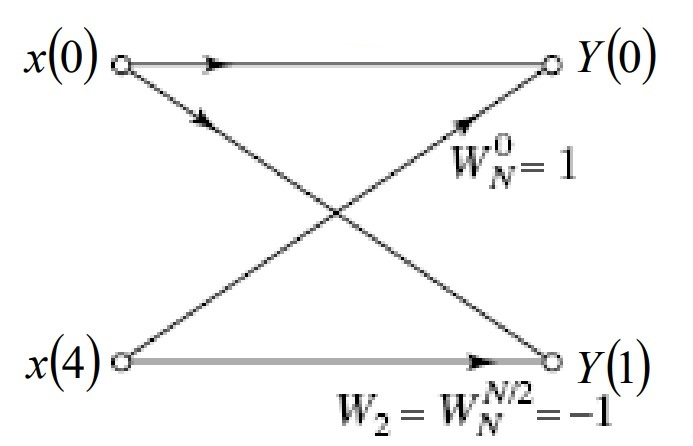
\includegraphics[width=4cm]{fft-dec-graph-bin}
		\caption{graph representation of the \fft using the decimation in time algorithm computed on 2 points.} \label{fig:dft:ditsing}
	\end{SCfigure}
	

	\begin{SCfigure}[2][bht]
		\centering 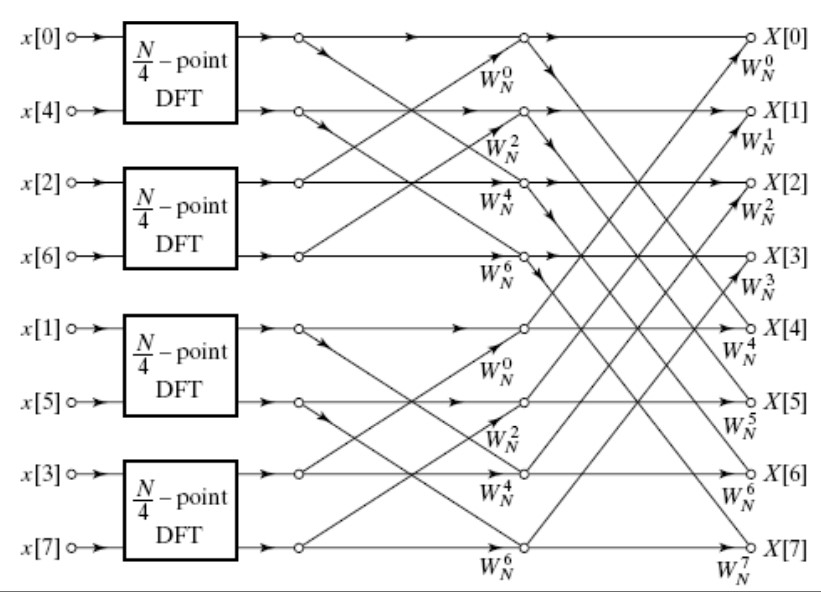
\includegraphics[width=7cm]{fft-dec-graph-comp}
		\caption{complete graph representing the computation to do with the decimation in time algorithm for $N=8$ samples. The transform of 2 value is shown in figure \ref{fig:dft:ditsing}.}
	\end{SCfigure}
	
	
	
	
	
	
	
	
	
	
	
	
	
	
	
	
	
	
	
	
	
	
	
	
	
	
	
	
	
	
	
	
	
	
	
	
	
	
	
	
	
	